% MIT License

% Copyright (c) 2019 Orange Lee

% Permission is hereby granted, free of charge, to any person obtaining a copy
% of this software and associated documentation files (the "Software"), to deal
% in the Software without restriction, including without limitation the rights
% to use, copy, modify, merge, publish, distribute, sublicense, and/or sell
% copies of the Software, and to permit persons to whom the Software is
% furnished to do so, subject to the following conditions:

% The above copyright notice and this permission notice shall be included in all
% copies or substantial portions of the Software.

% THE SOFTWARE IS PROVIDED "AS IS", WITHOUT WARRANTY OF ANY KIND, EXPRESS OR
% IMPLIED, INCLUDING BUT NOT LIMITED TO THE WARRANTIES OF MERCHANTABILITY,
% FITNESS FOR A PARTICULAR PURPOSE AND NONINFRINGEMENT. IN NO EVENT SHALL THE
% AUTHORS OR COPYRIGHT HOLDERS BE LIABLE FOR ANY CLAIM, DAMAGES OR OTHER
% LIABILITY, WHETHER IN AN ACTION OF CONTRACT, TORT OR OTHERWISE, ARISING FROM,
% OUT OF OR IN CONNECTION WITH THE SOFTWARE OR THE USE OR OTHER DEALINGS IN THE
% SOFTWARE.

\section{我的第一个 UWP 程序——Hello World}

\subsection{我需要会什么}

我们假设你会基于 ISO C++17 标准的 C++。其余内容,我们会在需要的时候学到。

\subsection{创建项目}

下面给出创建项目的详细步骤。

\begin{enumerate}
    \item 打开 Visual Studio 2019,选择``创建新项目''。
    \begin{figure}[htbp]
        \centering
        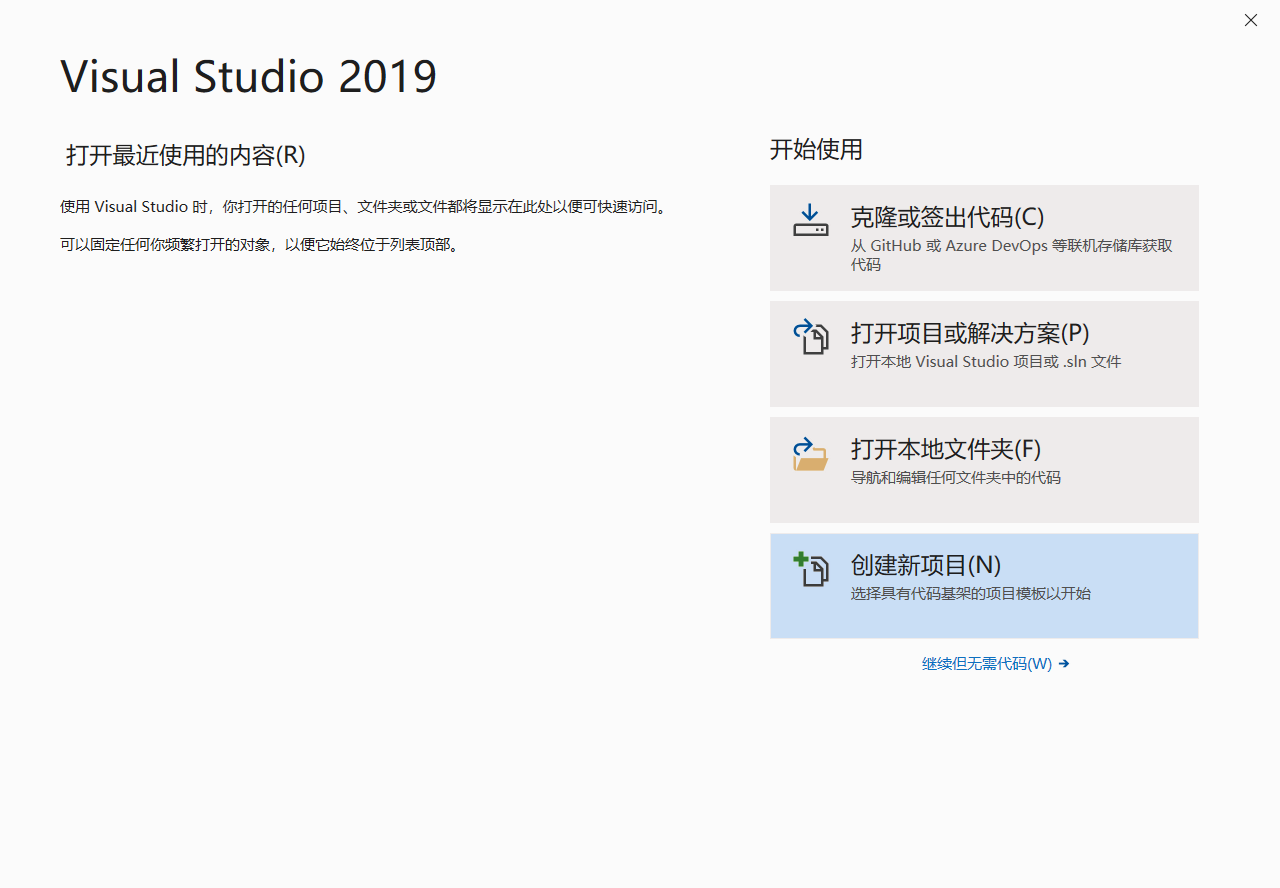
\includegraphics[width = 0.5\paperwidth]{pic/2.png}
        \caption{创建新项目}
    \end{figure}

    \item 选择``空白应用(通用 Windows - C++/CX)'',点击``下一步''。
    \begin{figure}[htbp]
        \centering
        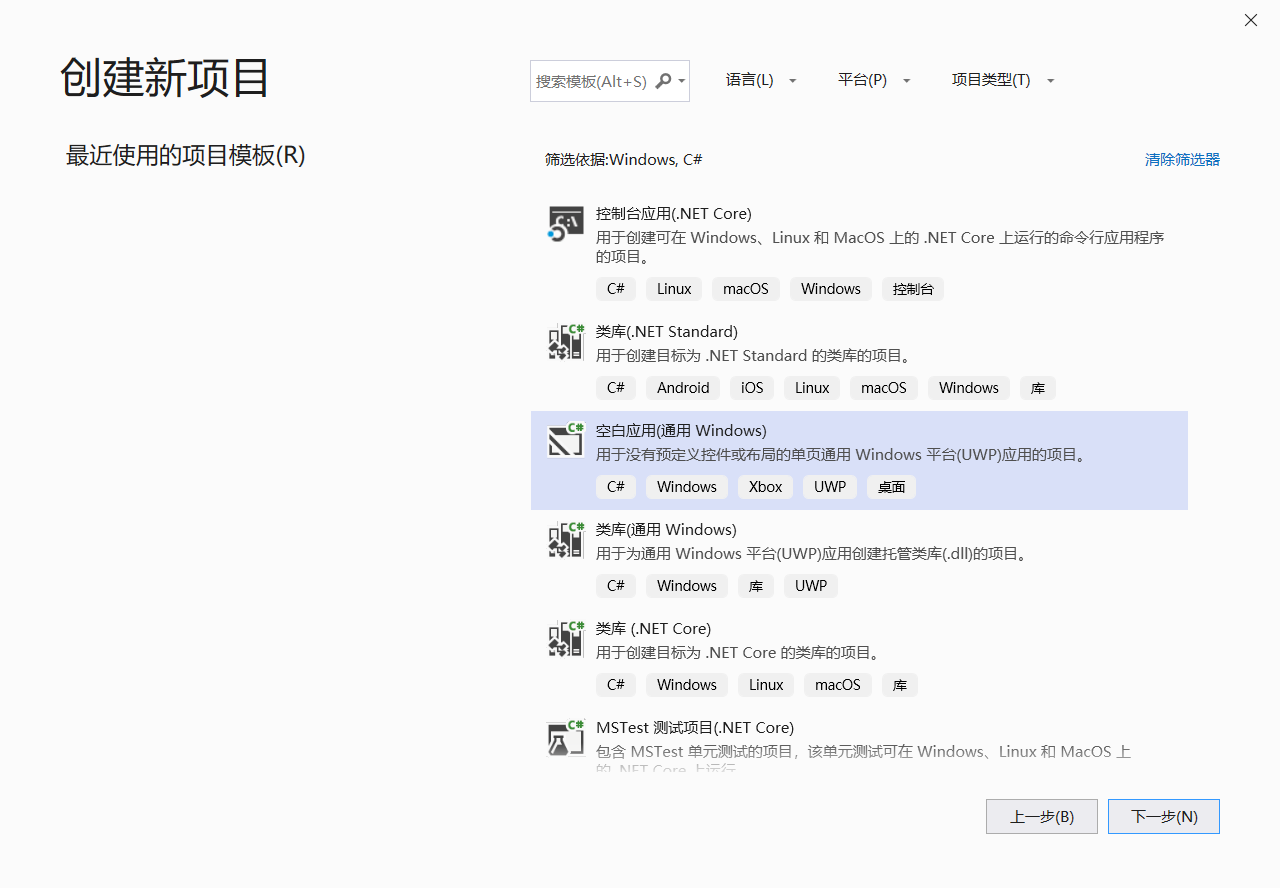
\includegraphics[width = 0.5\paperwidth]{pic/3.png}
        \caption{空白应用(通用 Windows - C++/CX)}
    \end{figure}

    \item 输入项目名称为``Hello World''。将鼠标悬浮在``解决方案名称''旁的信息图标上,可以看到``解决方案是 Visual Studio 中一个或多个项目的容器''。在这里我们只会创建一个项目,因此最好是勾选``将解决方案与项目放在同一目录中'',这样可以减少存放解决方案的文件夹的嵌套,对于小项目来说更便于管理。

    使用默认位置即可,直接点击``创建''。
    \begin{figure}[htbp]
        \centering
        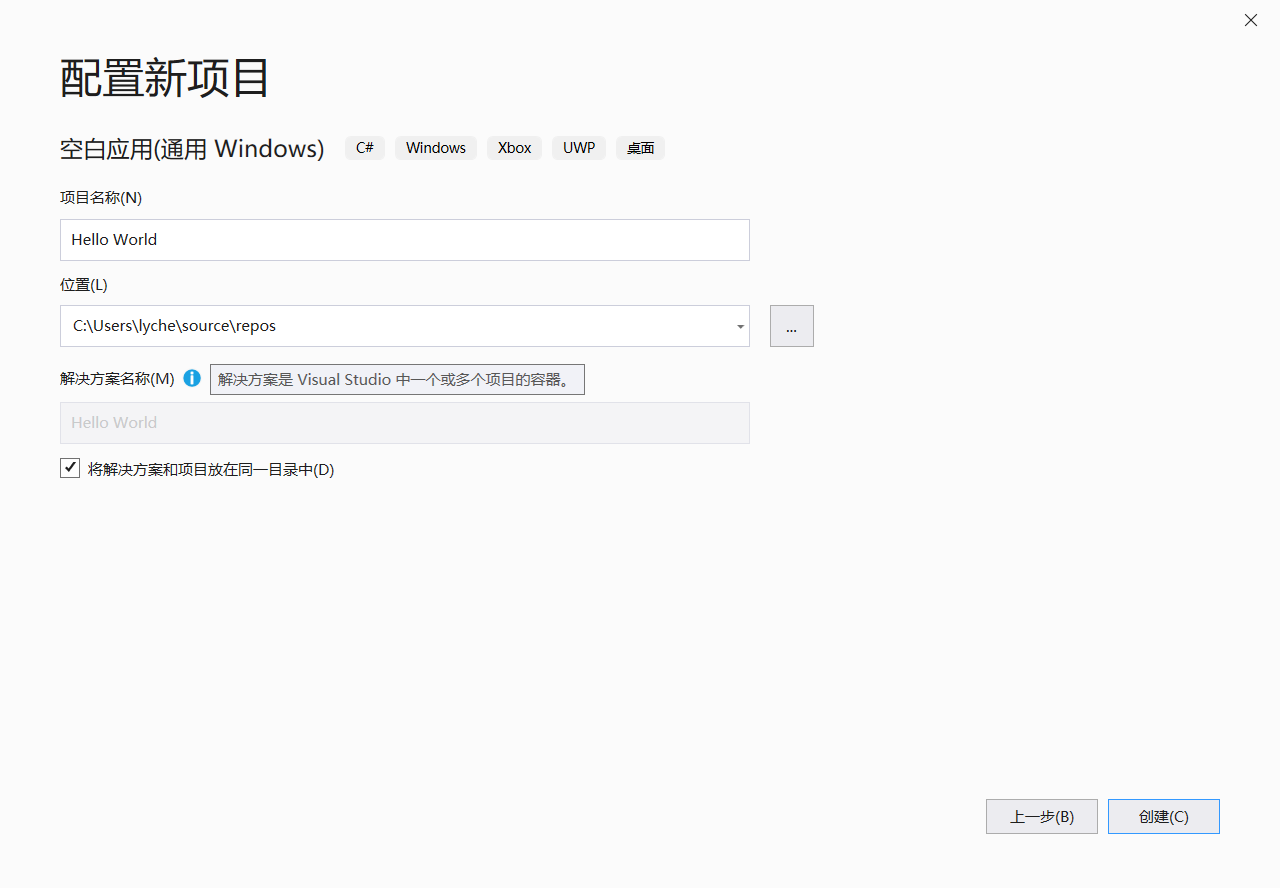
\includegraphics[width = 0.5\paperwidth]{pic/4.png}
        \caption{项目名称为``Hello World'',选中复选框,点击创建}
    \end{figure}

    \item 选择目标平台版本。新版本有新的特性,可以点击``我应选择哪个版本?''转到\href{https://docs.microsoft.com/zh-cn/windows/uwp/updates-and-versions/choose-a-uwp-version?ocid=VSClient_VerX_NewProject_version}{网页}查看每个版本对应的新特性。Hello World 当然不会用到这些新特性,所以我们直接点击确定即可。

    注意,这里假设你已经安装了最新版本的 Windows 10!
    \begin{figure}[htbp]
        \centering
        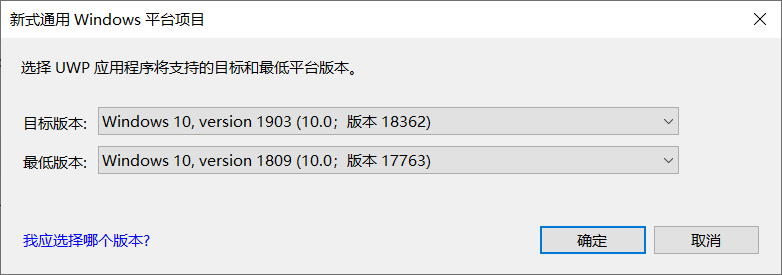
\includegraphics[width = 0.5\paperwidth]{pic/5.png}
        \caption{点击确定}
    \end{figure}
\end{enumerate}

至此,项目创建成功,我们进入到了 Visual Studio 的主界面。

\begin{figure}[htbp]
    \centering
    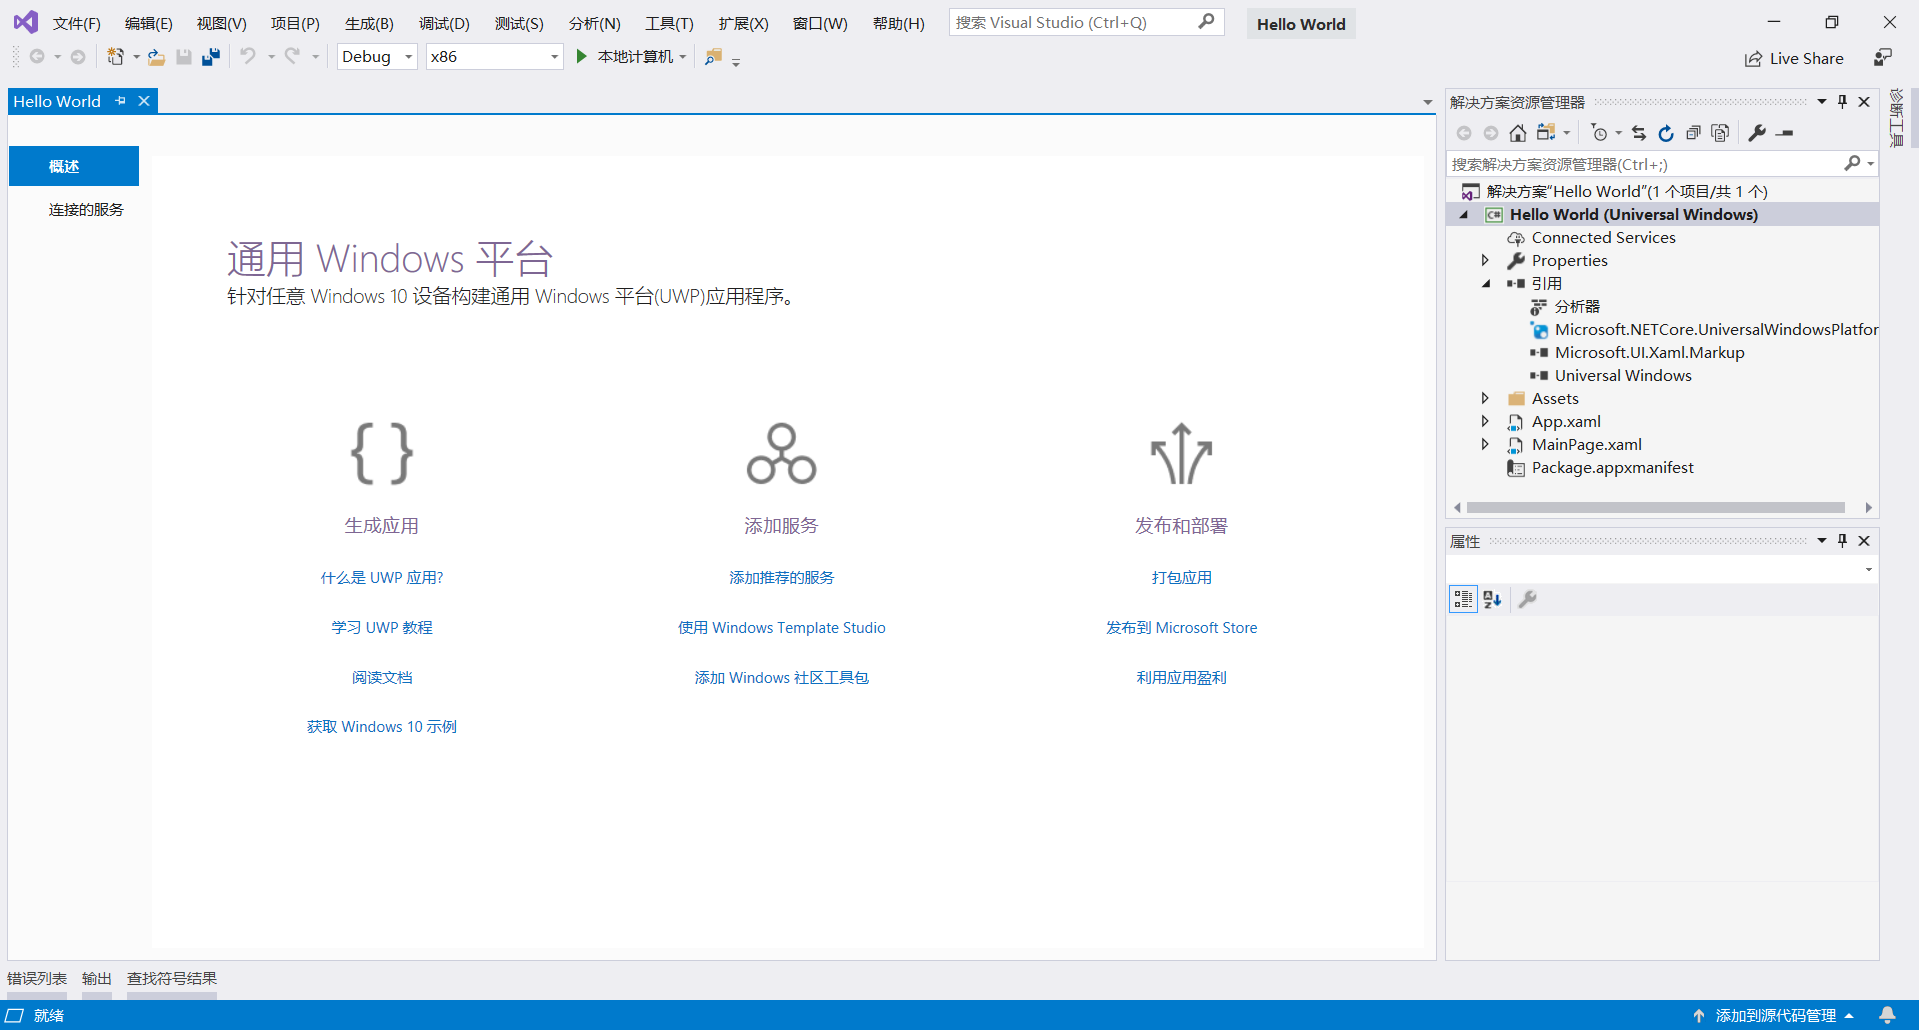
\includegraphics[width = 0.75\paperwidth]{pic/6.png}
    \caption{Visual Studio 主界面}
\end{figure}

你可能会注意到在创建项目完成后 VS 立马给你反馈了一些错误信息(如图)。不要担心,这是因为 VS 的 IntelliSense 还在加载;IntelliSense 负责进行代码提示,例如语法错误提示、代码补全等等。注意到状态栏最左侧的平行四边形了吗?如果里面有动画出现,说明正在运行后台任务,而 IntelliSense 的加载便属于其中一员。稍等片刻,便可以看见错误消失,状态栏左侧的平行四边形也没有了动画,点击后会提示你``没有后台任务运行''。

\begin{figure}[htbp]
    \centering
    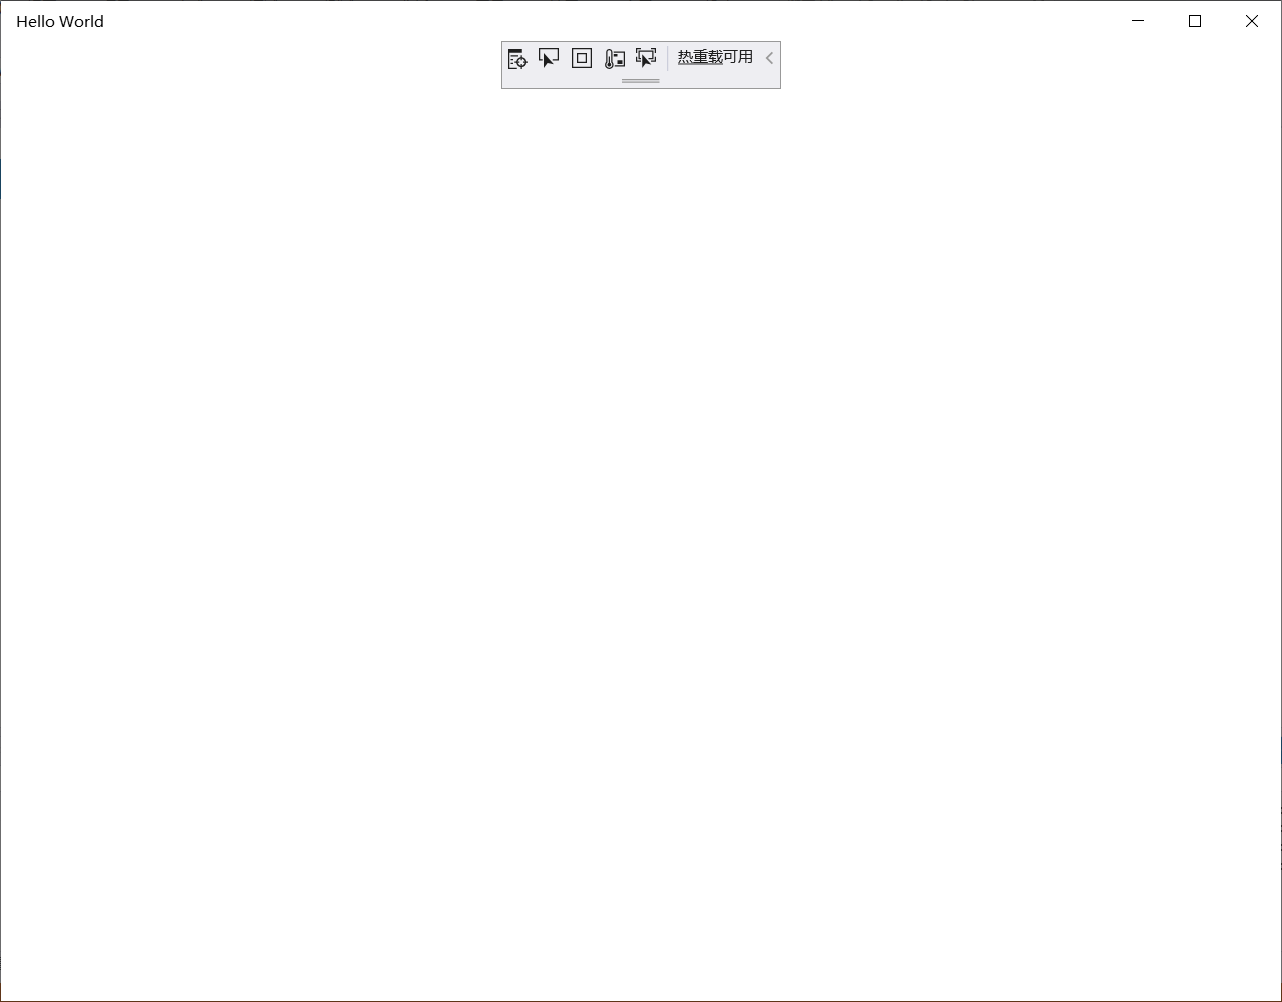
\includegraphics[width = 0.75\paperwidth]{pic/7.png}
    \caption{加载完成后的 Visual Studio 主界面}
\end{figure}

刚创建好的项目应该可以直接生成(build)并运行。我们尝试点击``{\Large$\triangleright$} 本地计算机'',等待编译完成后,可以看到程序已经运行。

\begin{figure}[htbp]
    \centering
    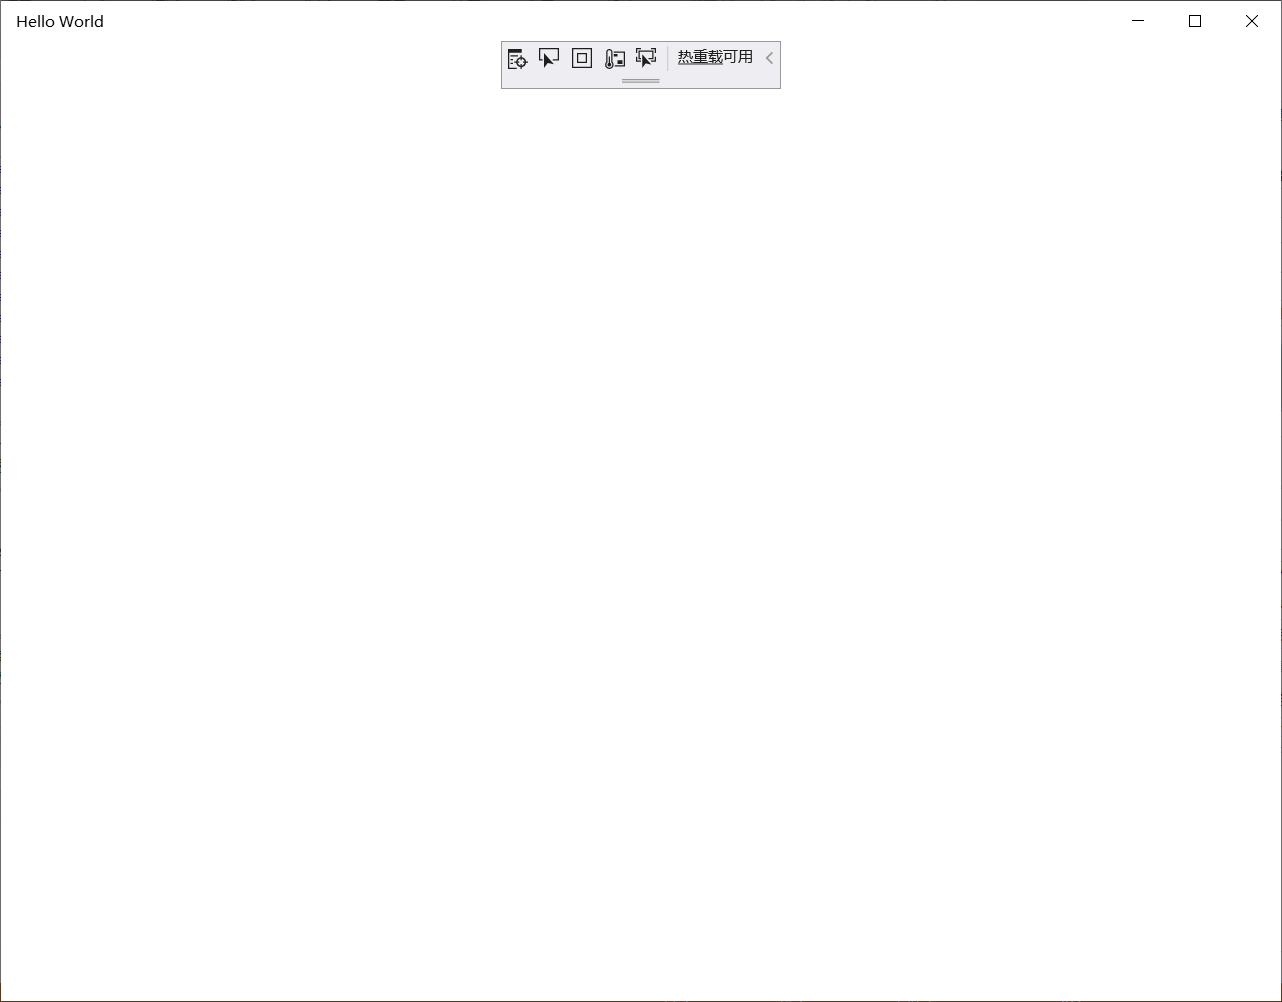
\includegraphics[width = 0.75\paperwidth]{pic/8.png}
    \caption{运行结果}
\end{figure}

可以发现,在 VS 中能够观察到程序的内存使用情况、CPU 使用情况等等,并且可以在 VS 中停止这个程序。这说明我们正在调试(debug)这个程序。以后我们可以始终可以通过点击``{\Large$\triangleright$} 本地计算机''或按下快捷键 F5 来调试程序。

还能在不调试的情况下启动程序。方法是在菜单栏中点击``调试''$\rightarrow$``开始执行(不调试)'',或直接按下快捷键 Ctrl + F5。

\subsection{解决方案资源管理器}\index{解决方案资源管理器}

解决方案资源管理器窗口是最重要的一个窗口之一。它给出了解决方案中所有项目的所有文件资源。
\begin{figure}[htbp]
    \centering
    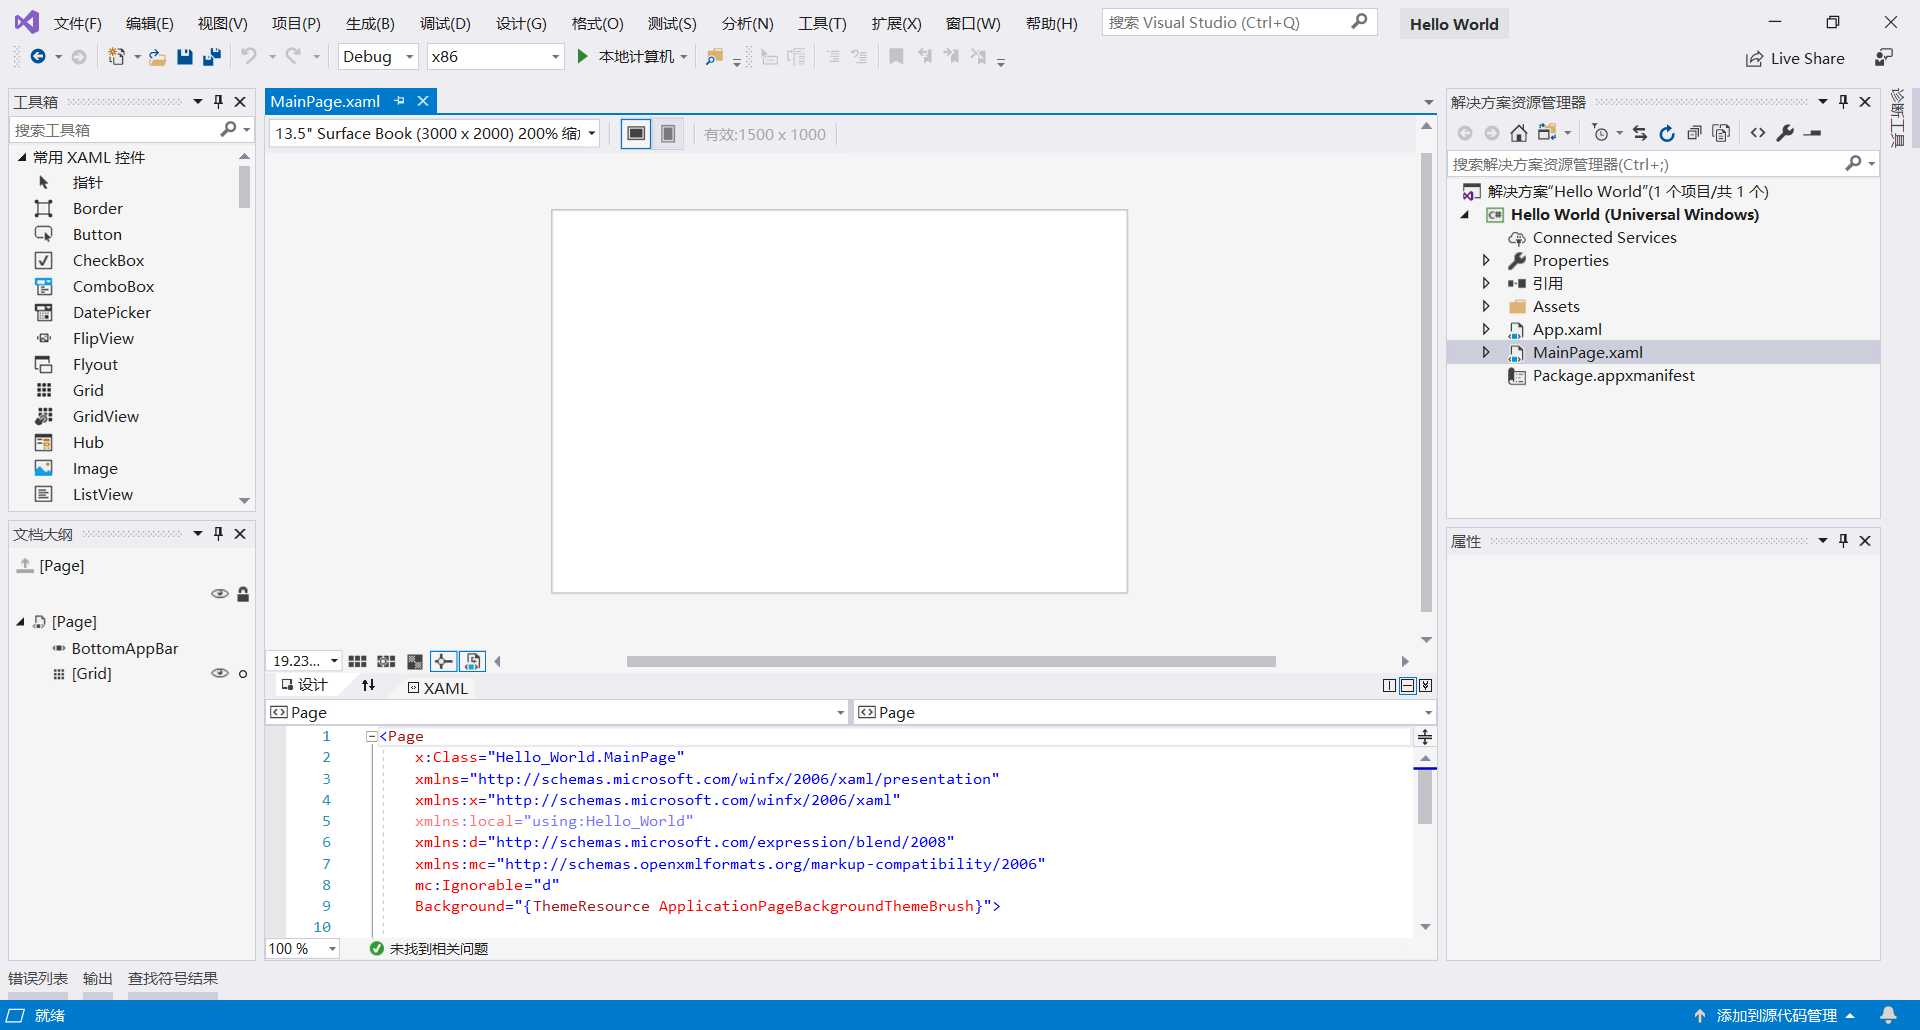
\includegraphics[width = 0.5\paperwidth]{pic/9.png}
    \caption{解决方案资源管理器}
\end{figure}

我们能大致看出这个项目的框架:这个项目使用 pch.cpp、pch.h 这两个文件进行预编译\index{预编译}\footnote{有关预编译的概念及作用,可以在网上搜索。},这个项目的相关属性在 Package.appxmanifest 中保存\footnote{manifest 是清单的意思,清单一般可以存放应用的相关信息。},这个项目的``主函数''在 App.xaml 下面的 App.xaml.cpp 中,这个项目有一个类似于窗口的东西,放在 MainPage.xaml 中……

目前,不明白每个文件的作用是很正常的事,现在我们也不用完全理解,我们只需要关注于如何写出 Hello World。

\subsection{Hello World 的开发历程}

双击解决方案资源管理器中的``MainPage.xaml'',可以进入如图 \ref{pic10} 所示界面。
\begin{figure}[htbp]
    \centering
    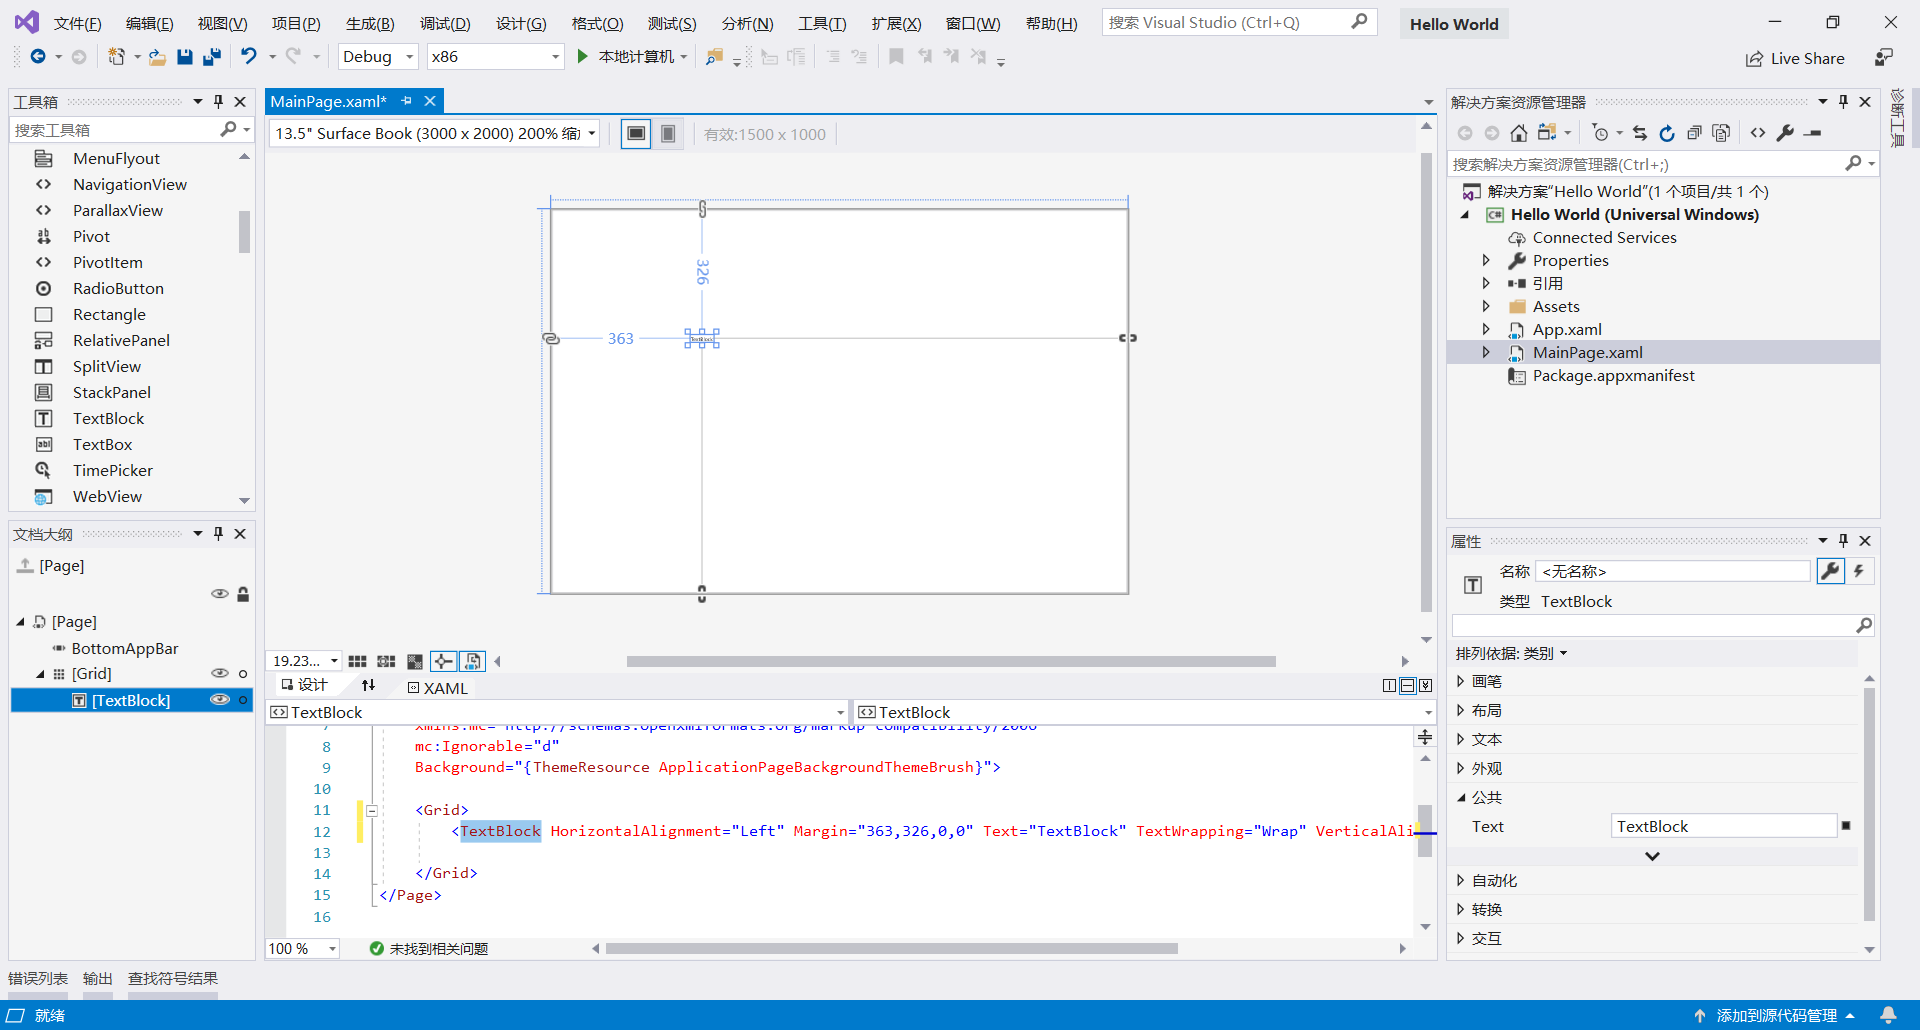
\includegraphics[width = 0.5\paperwidth]{pic/10.png}
    \caption{MainPage.xaml}
    \label{pic10}
\end{figure}

很显然这是一个窗口设计器。但可能会让你疑惑的是,当前窗口由两部分组成:上半部分是可视化设计器,下半部分是代码。我们不管这么多,为了尽早完成 Hello World,我们决定使用\textbf{工具箱}\index{工具箱}。

可以通过工具箱为窗口添加\textbf{控件}\index{控件}。这种工作方式在编写 Win32 程序时是很方便的,对于现在而言,我们写 Hello World 时使用工具箱也是很方便的。我们选中名为``TextBlock''的控件,将它拖动到可视化设计器中。
\begin{figure}[htbp]
    \centering
    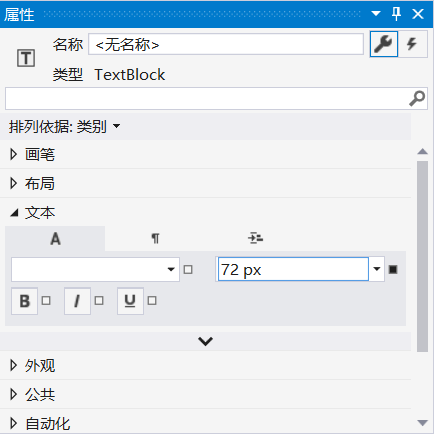
\includegraphics[width = 0.5\paperwidth]{pic/11.png}
    \caption{拖动 TextBlock 控件至可视化设计器中}
\end{figure}

可以看见,对于目前设计器的窗口大小而言,我们的 TextBlock 太小了。可以通过\textbf{属性窗口}找到更改这个 TextBlock 大小以及显示的文字的方法。
\begin{figure}[htbp]
    \centering
    \begin{minipage}[t]{0.4\paperwidth}
        \centering
        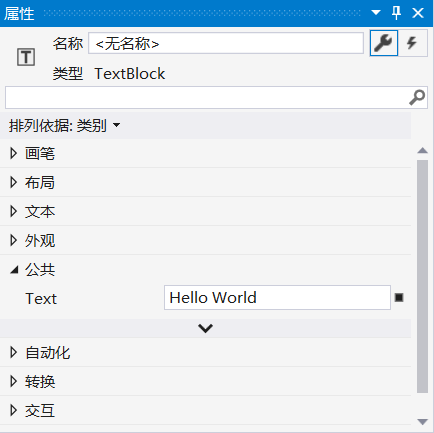
\includegraphics[width = 0.3\paperwidth]{pic/12.png}
        \caption{通过属性窗口更改 TextBlock 的显示内容}
    \end{minipage}
    \begin{minipage}[t]{0.4\paperwidth}
        \centering
        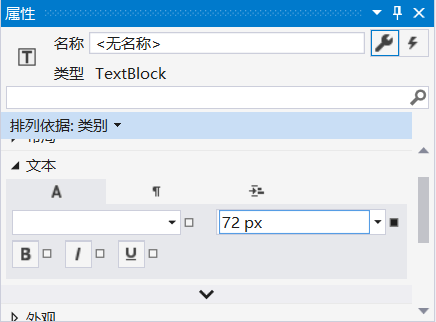
\includegraphics[width = 0.3\paperwidth]{pic/13.png}
        \caption{通过属性窗口更改 TextBlock 的字体大小}
    \end{minipage}
\end{figure}

最后,将 TextBlock 拖动到可视化设计器的左上角,按下 F5 调试,得到如图 \ref{pic14} 的结果。大功告成!
\begin{figure}[htbp]
    \centering
    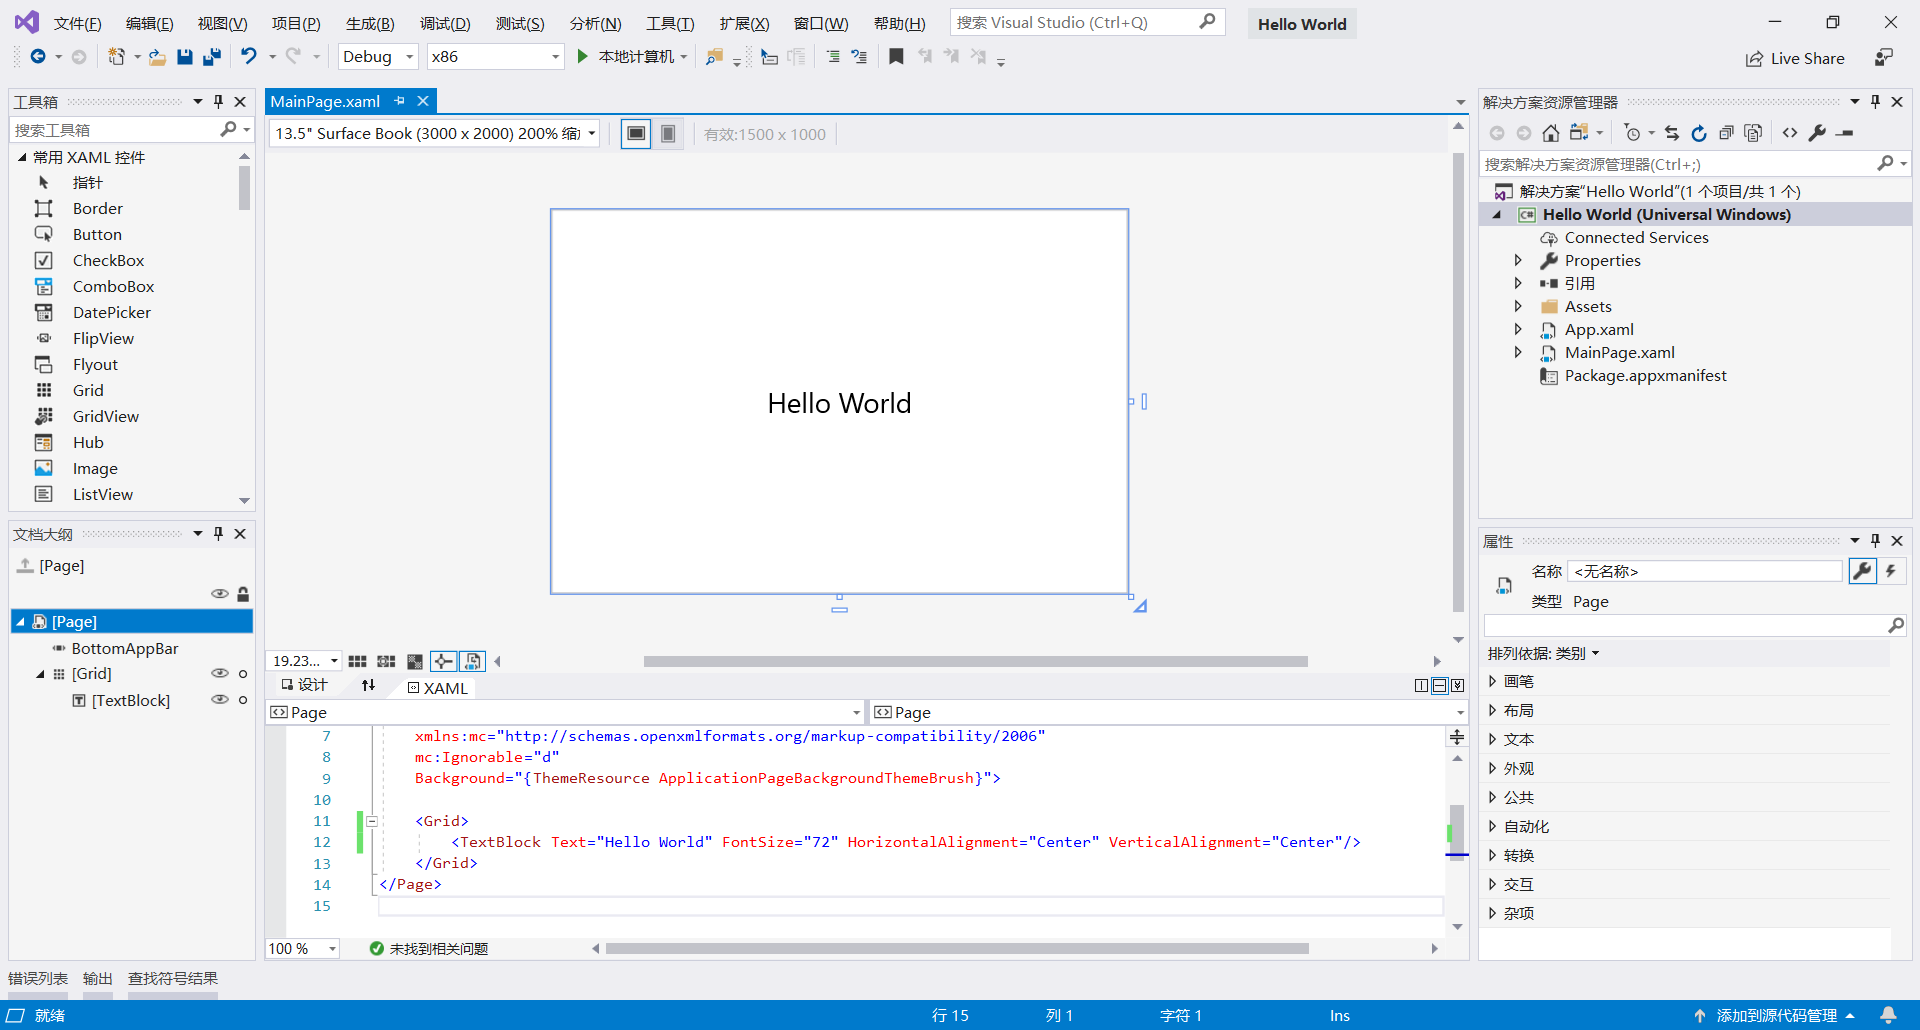
\includegraphics[width = 0.5\paperwidth]{pic/14.png}
    \caption{Hello World!}
    \label{pic14}
\end{figure}

\subsection{打包我的程序}

可以将你的程序打包成安装包的形式。点击菜单中的``项目''$\rightarrow$``应用商店''$\rightarrow$``创建应用程序包''。

要创建适合发布的安装包,我们将在以后讨论,这里只告诉你一个入口。

\subsection{笔记带有源代码吗?}

有!就在 UWP projects 目录下!